\documentclass[12pt]{article}
\usepackage{graphicx} % Required for inserting images

\title{Lab 01: Introduction to Lab Equipment
}
\author{Owen Strong \\
\itshape Prof.: Angela DiFulvio\\
\itshape TA: Kholod Mahmoud \\
\itshape TA: Schaffer Bauer \\
}
\date{7 February 2026}

\usepackage[
    style=ieee
]{biblatex}
\bibliography{refs.bib}

\usepackage[letterpaper, margin=1in]{geometry}
\newcommand{\figwidth}{0.75\linewidth}
\begin{document}

\maketitle
\begin{abstract}
    Before performing experiments, it is crucial to have a comprehensive understanding of the equipment used. 
    In this laboratory, we perform a series of experiments to build this understanding. 
    In experiments 1 and 2, we connect a pulser to an oscilloscope to familarize with controls of both: practicing viewing signals on the oscilloscope and producing controlled signals on the pulser.
    In experiment 3, we replicate  a typical system to process the signal from a radiation detector to build understanding of a preamplifier and amplifier, and compare the effect of different gain settings, shaping settings, and the single-channel-analyzer (SCA) output.
    In experiment 4, we mimic the setup of a radiation counter by measuring the pulses of a pulser, to familiarize with the usage of a timer-counter.
    In experiment 5, we repeat the signal processing system of experiment 3, and further familiarize with an amplifier by observing the discrimination parameters necessary to discriminate noise or to falsely discriminate the intended pulser signal.\\

    We demonstrate ability to use the pulser to produce controlled sample pulses, the oscilloscope to view and measure repeating pulses, the preamplifier and amplifier to enhance, amplify, shape, and discriminate pulses, the timer-counter to count signals over a time period, and BNC cables to connect different components.
    We record the effects of different controls for the oscilloscope.
    We record sample waveforms from the pulser directly, then with the preamplifier and amplifier processing pulser signal, with different configurations of gain and shaping from the amplifier.
    We generate an SCA pulse with a measured width of 8 microseconds, magnitude 0.8875V, and frequency 60.06Hz, compared to a corresponding amplified pulse of 21 microseconds, 100mV, and identical 60.06Hz.
    Using the timer-counter, we measure 3598 pulses in 60 seconds, an extremely similar frequency of 59.96Hz.
    We find a much more reliable control over amplification with the amplifier ($R^2=0.999$) than using the Pulser gain and Preamplifier directly ($R^2=0.574$).
    We find that for an SCA pulse of amplitude 0.8825V, a lower-level discriminator of at most 0.26, or separately an upper-level discriminator of at most 0.06 were required to guarantee false discrimination of the target signal.\\

    These results will allow the proper usage of the tested Nuclear Instrumentation Module standard devices to form nuclear instrumentation systems in the future, and debug them where necessary using an oscilloscope.
\end{abstract}

\section{Introduction and Background}

A variety of equipment is involved in radiation detection, and particularly in designing experiments for this purpose.
An intimate knowledge of the equipment used is therefore crucial to performing experiments quickly and effectively, as well accurately and reproducibly describing them. \\

In order to clearly and reproducibly perform experiments, the required system is broken up into discrete components, or modules, which fit onto a module rack.
These modules are designed according to the Nuclear Instrumentation Module (NIM) standard to allow greater flexibility and ease for design and update.
Examples of NIM devices may be found in Figure~\ref{fig:intr-modules}
\begin{figure}[!htb]
    \centering
    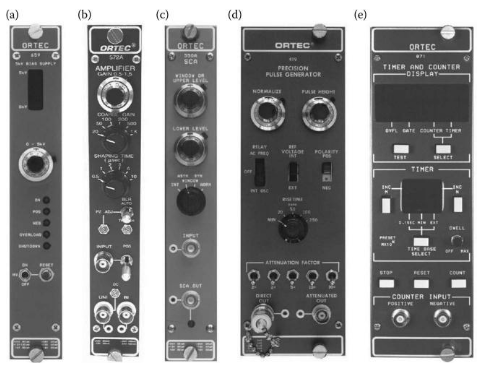
\includegraphics[width=\figwidth]{figs/Int0_Modules.png}
    \caption{Typical commercial NIM devices: (a) HV power supply, (b) amplifier, (c) single-channel analyzer, (d) scaler, (e) timer and counter (Sourced from Textbook\cite{tsoulfanidis_measurement_2015}, original from Advanced Measurement Technology—ORTEC)}
    \label{fig:intr-modules}
\end{figure}
In this laboratory, we consider the common workhorse equipment of future experiments: a module rack, pulser, preamplifier, amplifier, and oscilloscope.
These modules may then be arranged in a reproducible system, with standardized connections and settings, which might be described in brief with a system diagram like in Figure~\ref{fig:intr-example-system}.
\begin{figure}[!htb]
    \centering
    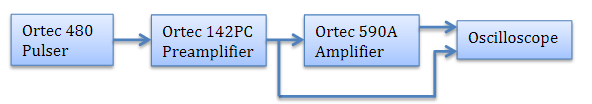
\includegraphics[width=\figwidth]{figs/Mat1_Exp3Setup.png}
    \caption{The system setup of experiment 3, as an example. At the start is the pulser, whose output is fed into an input of the preamplifier. One output from the preamplifier is taken, then fed using a t-splitter cable into both the input of an amplifier and one input channel of an oscilloscope. An output from the amplifier is then fed into the oscilloscope. Sourced form the Lab Manual~\cite{npre_lab_1_manual_2025}}
    \label{fig:intr-example-system}
\end{figure}
This diagram serves as a broad reference on the character of experimental measurement.
Further details on exactly which connectors on each module are used, and how each module is configured, would be elaborated upon in the experimental description.
\\

\subsection{Pulser}
Since experimental output can be unpredictable (After all, we need to run the experiment to find out!), several common components revolve around debugging sensors prior to, or even during, experimental procedures.\\

The first such tool we will describe is the pulser.\\

Electronic instrumentation typically outputs signal pulses which are fed into a circuit constructed on a NIM rack.
The pulser, therefore, outputs a predictable and programmable signal output simulating that which an experimental detector could produce.
In this way, the behavior of the successive circuit may be explored in a controlled fashion.\\

This laboratory intends to demonstrate ability to connect a pulser to a system and configure its output amplitude, attenuation, and polarity.
Experiment 1 introduces the pulser, but all five experiments make use of it to some extent.
\\

\subsection{Oscilloscope}

Another key tool to analyze signal output is the oscilloscope.
An oscilloscope displays the output of a voltage signal, and is particularly designed to analyze rapidly repeating signals such as from a pulser. 
An oscilloscope displays some section of an input signal, and using a configurable Trigger (e.g., when the rising edge of a signal crosses a threshold 0.5V), resets the view to center on every new pulse to observe the overall repeating wave. 
The oscilloscope is thus a very useful tool to visualize the output of an instrument processing system, particularly when being debugged by using a pulser as an input.\\

Experiment 1 introduces the oscilloscope, and focuses on the ability to manipulate the view of a particular model of oscilloscope.
Experiments 2, 3, and 5 additionally use the oscilloscope.


\subsection{Cables}
Several types of cables may be used in laboratories, but in this lab the most common, BNC cables are used.\\

BNC cables may be used for most purposes, except to carry high voltage signals\cite{npre_lab_1_manual_2025}, for which an SHV or MHV cable may be used instead.
The three cables may be compared in Figure~\ref{fig:mat-cables}, and in particular the similarity between BNC and MHV connectors. Special care should be taken to avoid mixing these cables, which are not compatible, to avoid damage.
In this laboratory, this concern may be alleviated by the exclusive use of BNC cables (after observing an SHV and MHV cable for comparison), but in future laboratories, the risk must be taken into account.\\
\begin{figure}[!htb]
    \centering
    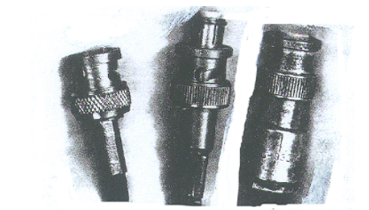
\includegraphics[width=\figwidth]{figs/Mat2_cables.png}
    \caption{From left to right: BNC, SHV, and MHV connections. Note the similarity between BNC and MHV connectors. Sourced from lab manual\cite{npre_lab_1_manual_2025}.}
    \label{fig:mat-cables}
\end{figure}

All experiments make use of BNC cables.\\


\subsection{Counter}

A typical quantity of interest in an experiment is simply the number of pulses a detector produces. At the tail end of a circuit where the signal has been processed into something simple like a logic pulse, this may be fed to a timer-counter device which tracks the number of pulses received within a set window of time.\\

Experiment 4 demonstrates output to a timer-counter device, reinforcing with comparison to prior experiments.\\

\subsection{Preamplifier}

The preamplifier serves as an optimized connection between the raw output of the detector and the rest of the experimental system.\cite{tsoulfanidis_measurement_2015}
The detector signal output may be very weak and full of noise, and will have to be amplified, sometimes by factors of thousands.
In order to preserve as useful a signal as possible, a preamplifier will be connected as closely to the detector as possible, and will shape the signal and account for attenuation, such that the signal may then be safely transmitted to the amplifier.
Because of this spacial requirement, a preamplifier such as the one used in this experiment might not fit in the Module Rack, instead being separate but attached to position near the detector.\\

Experiment 3 introduces a preamplifier, and builds familiarity with its output signal.
Experiments 4 and 5 make similar use of the preamplifier.\\


\subsection{Amplifier}
Once a signal has been preserved by the Preamplifier, it may then be amplified by an amplifier to achieve a measurable magnitude.
The amplifier can magnify signals by factors of a thousand or more, but is still limited in its overall output, typically to 10V.\cite{tsoulfanidis_measurement_2015}.
It is thus key to properly configure the gain of the amplifier to allow all expected outputs to fit within an expected and measurable voltage range.\\

Experiment 3 introduces an amplifier in conjunction with the preamplifier, comparing their signals and demonstrating configuration of its gain and shaping parameters. Experiments 4 and 5 make similar use of the amplifier.\\


The rest of this report proceeds as follows: In Section~\ref{sec:methods}, the specific equipment used will be described, followed by the experiments performed using them.
Section~\ref{sec:results} describes the results found in detail, Section~\ref{sec:disc} discusses the implications of these results, and Section~\ref{sec:conc} furnishes an overview of the laboratory and its significance.


\section{Experimental Procedure}\label{sec:methods}
This section describes the components used in this laboratory, which will be used in many future experiments.
\\

\subsection{Module Rack}

In this experiment, a Canberra Model 2000 module rack was used (inventory number NE759377), as depicted in Figure~\ref{fig:mat-mod-rack}. This component will be henceforth referred to as the Module Rack.
\begin{figure}[!htb]
    \centering
    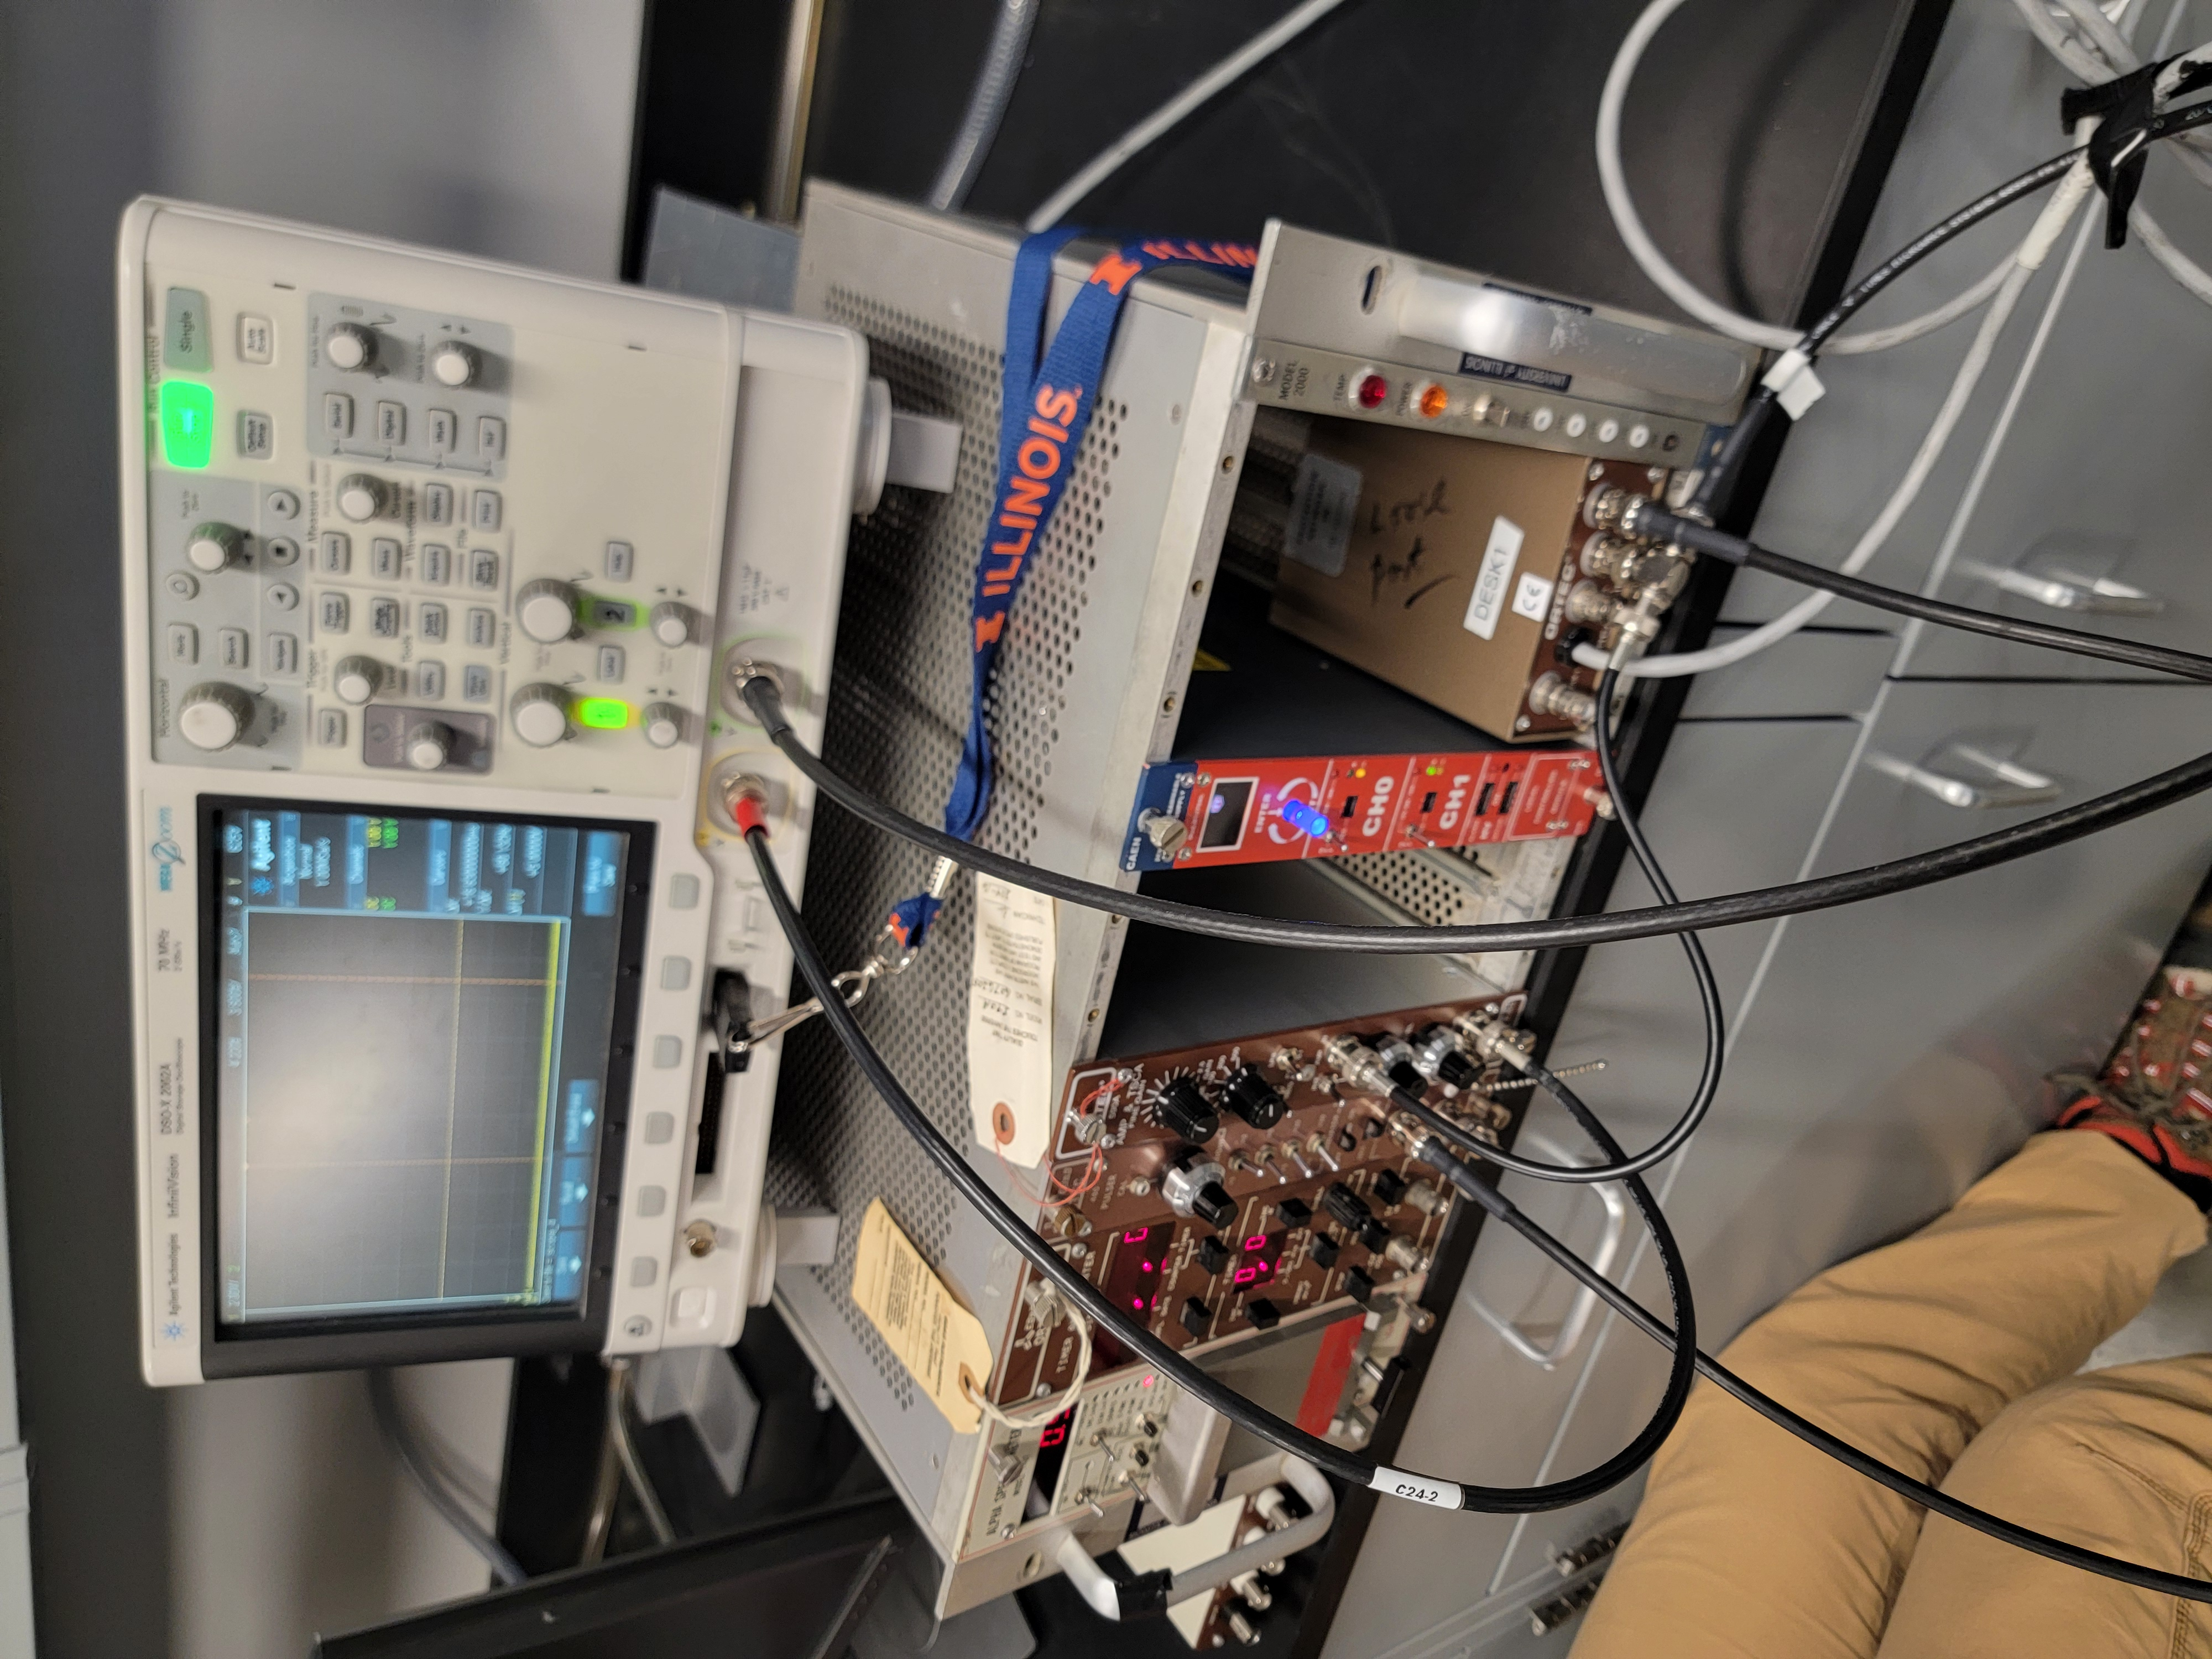
\includegraphics[width=\figwidth,angle=270]{figs/Mat0_ModuleRack.jpg}
    \caption{The Canberra Model 2000 NIM rack used in this lab. Additionally visible are the modules within it as used in this laboratory. From left to right: a Canberra Model 7401 Alpha Spectrometer (unused), an Ortec Model 871 Timer-Counter (used, serial \# 1024), an Ortec Model 480 Pulser, an Ortec Model 590A AMP \& TSCA (used, serial \# 16076205), a Caen N1470AL Programmable Power Supply (unused, property \# P10G96054), and an Ortec 142PC Preamplifier (used, serial \# 2780, revision 17, not directly attached to the NIM rack). The components are attached to each other using BNC cables of varying lengths. Atop the rack lies an Infiniivision DSO-X 2002A Oscilloscope (used, inventory \# P10R03513).}
    \label{fig:mat-mod-rack}
\end{figure}

\subsection{Pulser}
In this laboratory, an Ortec Model 480 Pulser was used, which may be seen in Figure~\ref{fig:mat-mod-rack}.
This particular pulser will henceforth be referred to as the Pulser, to distinguish from pulsers in general.
A serial number tag was not attached externally, and the module could not be removed to identify the Illinois property number on its side.


\subsection{Oscilloscope}

In this laboratory, an Infiniivision DSO-X 2002A Oscilloscope (inventory \# P10R03513) was used, which may be seen on top of the module rack in Figure~\ref{fig:mat-mod-rack}.
The particular oscilloscope used in this experiment will henceforth be referred to as the Oscilloscope.


\subsection{Counter}

In this laboratory, an Ortec Model 871 Timer-Counter (serial \# 1024) is used, which may be observed in Figure~\ref{fig:mat-mod-rack}, which will henceforth be referred to as the Counter.

\subsection{Preamplifier}
In this laboratory, an Ortec 142PC preamplifier (serial \# 2780, revision 17) is used, henceforth referred to as the Preamplifier.
No Illinois property number was identifiable on the Preamplifier.

\subsection{Amplifier}

In this laboratory, an Ortec Model 590A Amplifier and Timing Single Channel Analyzer (AMP \& TSCA, serial \# 16076205), seen in Figure~\ref{fig:mat-mod-rack} was used, and is henceforth referred to as the Amplifier.

\subsection{Experiment 1: General Oscilloscope Observation}
Experiment 1 familiarizes the user with the Oscilloscope and BNC cables.\\

A BNC, SHV, and MHV cable are observed to ensure lab operators can visually distinguish the types. Using a BNC cable, we connect the Pulser to the Channel 1 input of the Oscilloscope, creating the system seen in Figure~\ref{fig:mat-exp1-setup}. 
We then spend time configuring various knobs on the Oscilloscope, to familiarize with it.
Namely, the "Auto Scale" button, "Trigger" knob, and the large and small "Horizontal" and "Vertical" knobs are tested.

\begin{figure}[!htb]
    \centering
    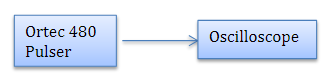
\includegraphics[width=\figwidth]{figs/Mat3_Exp1Setup.png}
    \caption{Setup for experiment 1. Sourced from Lab Manual.\cite{npre_lab_1_manual_2025}}
    \label{fig:mat-exp1-setup}
\end{figure}


\subsection{Experiment 2: Pulser Output}
Experiment 2 familiarizes with the Pulser, using the same experimental setup as in experiment 1.
The Pulser has two outputs, both direct and attenuated. The direct output produces repeating pulses with amplitude adjusted by the "Pulse Height" dial on its face, and the attenuated output is reduced by a certain fraction. This experiment compares the two.\\

Using a BNC cable, the Pulser is connected at its DIRECT OUTPUT port to Channel 1 on the oscilloscope.
We adjust the Pulse Height dial fully clockwise, and set the output polarity switch to positive.
We then, using the large vertical and horizontal knobs, adjust the vertical scale of the Oscilloscope to 1 V per division, and the horizontal scale to 100 microseconds per division, and set all attenuators to "x1".
We use the Trigger knob as found in experiment 1 to adjust the Trigger to leading edges at approximately 50\% the observed magnitude of Pulser waves, and using the small vertical and horizontal knobs, translate the view of the oscilloscope to a waveform, using the large knobs to rescale it as necessary to view just one complete waveform. We use the Measure knob (pressing to switch between different vertical and horizontal markers, and rotating to move those markers across the view window) to measure the amplitude of the pulses by moving one y marker to the observed baseline and the other to the observed peak, and recording the difference between the two.\\

After adjusting the horizontal scale to view multiple pulses again, the x markers are likewise used to measure the time between two pulses, and record this time $t$ and the associated frequency $f=t^{-1}$. \\

We then move the BNC cable from the DIRECT OUTPUT channel of the Pulser to the channel labeled ATTEN OUTPUT. We observe the properties of this pulse on the Oscilloscope as with the DIRECT OUTPUT, then repeat these observations again and compare after flipping the attenuation to "2x". 

\subsection{Experiment 3: Preamplifier and Shaping Amplifier.}
This experiment replicates a typical system from the output of a radiation detector to an end output like a counter or spectrometer. The general form may be observed in Figure~\ref{fig:mat-exp3-setup2}.\\

\begin{figure}[!htb]
    \centering
    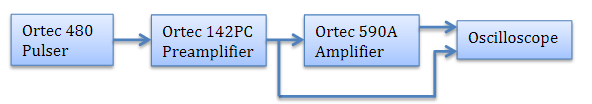
\includegraphics[width=\figwidth]{figs/Mat1_Exp3Setup.png}
    \caption{The setup of experiment 3. Sourced from Lab Manual\cite{npre_lab_1_manual_2025}}
    \label{fig:mat-exp3-setup2}
\end{figure}
We first consult with the Lab TA for assistance connecting the Preamplifier to the power supply in the back of the cable, as this special procedure does not use one of the three familiar cable types.\\
We then connect the components to form the system shown in Figure~\ref{fig:mat-exp3-setup2} using BNC cables.
We route the pulser ATTEN OUTPUT to the TEST port on the Preamplifier, the ENERGY (E) output on the Preamplifier to a BNC-tee, or t-splitter, to the INPUT port on the Amplifier, and the AMP output of the Preamplifier to Channel 1 of the Oscilloscope. Using the other output of the t-splitter, we also connect ENERGY on the Preamplifier directly to Channel 2 of the Oscilloscope.\\
We adjust the Pulser pulse height and attempt to have the direct Preamplifier output an amplitude of around 25mV. We set the gain of the amplifier to its smallest value (0.5 fine, 10 coarse), and set the shaping switch to UNIPOLAR (as opposed to BIPOLAR).\\
We compare the direct Preamplifier and the post-Amplifier signals on the Oscilloscope, and record to a flash drive.
Then, we repeat these observations and compare after setting the shaping switch to BIPOLAR.\\
To quantify the effect of Pulser gain, we hold the Amplifier gain settings constant, and choose four pulse height settings (1.74, 2.6, 3.8, 5) on the Pulser, using the Measure dial as described in experiment 2 to measure the amplitudes from baseline to peak of Direct and Amplifier output pulses on the Oscilloscope.\\
Likewise, to quantify the effect of Amplifier gain, we hold the Pulser's pulse height setting constant at 1.74, and pick four different Amplifier gain values (constant 0.5 fine gain and 10x, 20x, 50x, and 100x coarse gain), recording the amplitudes of just Amplifier pulses, as only Amplifier settings are changed.\\

Then, to investigate SCA output, we return the Amplifier gain to its lowest value and adjust Pulser gain, this time to reach an Amplifier output signal as close to 100mV as possible. We ensure the SCA switch is set to INT, not WINDOW, and adjust both SCA knobs to a minimum of 1.0. We connect the cable from the Preamplifier output to the Oscilloscope to instead connect the SCA output of the Amplifier to the Oscilloscope, such that the AMP and SCA outputs of the Amplifier may be compared thereupon. Adjusting the Oscilloscope viewport as necessary, we use the Measure dial as previously described to measure the pulse width, frequency, and amplitude of the SCA output signal.

\subsection{Experiment 4: The Timer-Counter}
This experiment mimics a basic setup to count radiation, such as a Geiger counter, and aims to familiarize with the Counter.\\
\begin{figure}[!htb]
    \centering
    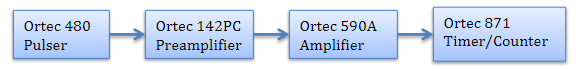
\includegraphics[width=\figwidth]{figs/Mat4_Exp4Setup.png}
    \caption{The setup of experiment 4. Sourced from Lab Manual.\cite{npre_lab_1_manual_2025}}
    % \label{fig:mat-exp4-setup}
    \label{fig:mat-exp4-setup}
\end{figure}
We first consult with the TA on how to configure the timer on the Counter.
Of the two displays on the Counter, the lower one located in the center of the Counter displays the timer length as digits M and N, where the timer length corresponds to $M\times10^N$. 
% The button directly below this display switches an "edit light" to be under either M or N, and the button to the left of the display increments whichever number the edit light is under.\\
The buttons adjacent to digits M and N increment their respective digit.\\
The top display displays either the time processed, or the number of signals observed in that time, and is toggled using the SELECT button under it to the right.\\
On the bottom row of the Counter, the COUNT button starts counting time and signals until either the selected time on the timer is measured or the STOP button is pressed to interrupt.
The RESET button resets both the timer and the count to 0.\\
We then configure the equipment as shown in Figure~\ref{fig:mat-exp4-setup}, using the AMP output of the Amplifier and ensuring it is set to UNIPOLAR. We set the timer on the Counter to count up to 60 seconds ($6\times10^1$), start the timer, and after the 60 seconds have passed record how many signals were counted, comparing to that expected (measured frequency $f [s^{-1}]\times60[s]$).

\subsection{Experiment 5: The Discriminator}
This experiment aims to familiarize with the discrimination options on an amplifier, to eliminate pulses which are too large or too small.
In the case of the Amplifier chosen, a lower-level discriminator (LLD) labeled "LOWER LEVEL", and upper-level discriminator (ULD) labeled "WINDOW" are available.
The Single Channel Analyzer (SCA, as labeled over its respective output channel on the Amplifier) yields a logical pulse when an input signal is above LLD and below $\mathrm{LLD+ULD}$.
This Amplifier may also be set to either WINDOW mode (as described above), or INT mode (which ignores ULD, effectively assuming $\mathrm{ULD=\infty}$).\\
We reuse the setup from experiment 3, as shown in Figure~\ref{fig:mat-exp3-setup2}, and connect both the AMP and SCA outputs of the Amplifier to the Oscilloscope.
We set the LLD to its minimum value and SCA to its highest, and the SCA to WINDOW mode.\\
Using the Pulser's gain, we generate an output pulse as close to 1.0V as can be generated. We increase the LLD value slowly until the signal begins to flicker on the Oscilloscope before finally disappearing completely, and record this LLD value. We then reset the LLD to its minimum, and slowly reduce the ULD value from maximum until the signal likewise flickers and disappears, recording these ULD values.
\section{Experimental Results}\label{sec:results}
% Experiment 1
% Written explanation
\subsection{Experiment 1: General Oscilloscope Observation}
The "Trigger" knob, when spun, was found to adjust the y level at which the display reset and centered repeating signals.
This was displayed by an orange horizontal line, which was shown while rotating the knob, and disappeared afterwards.
Pressing the knob was found to set this value to approximately halfway between the minimum and maximum observed y values in some recent timespan, again briefly showing it with a horizontal orange line.
The large "Vertical" and "Horizontal" knobs were found to zoom in or out on the vertical (voltage measurement) and horizontal (time) axes. 
The small knobs were found the window to pan across their respective axes.\\
The "Auto Scale" button was found to, as suggested, automatically frame the repeating signal.
The oscilloscope ceased graphing for a few seconds while presumably performing calculations, then the reframed repeating signal was displayed.
The Trigger was automatically set to some intermediate value of voltages recorded, such that in most cases the display correctly centered on a waveform.
The time scale (horizontal) and amplitude scale (vertical) were adjusted so the highest and lowest points of the target waveform fit comfortably in the screen, and multiple wave patterns were visible simultaneously.
% Experiment 2
% Sample pulse, for attenuated wave and directly acquired.
\subsection{Experiment 2: Attenuated and Directly Acquired Waveforms}
Adjusting the Trigger manually yielded noticeable effect: When the trigger value was raised to higher than the pulse height, the Oscilloscope was unable to center on the repeating waveform, and the waves proceeded across the screen in a messy blur.
Setting the Trigger to approximately half the pulse height on the rising edge of the pulse resolved this issue, and allowed the Oscilloscope to properly center on the repeating waveform.
\\
After adjusting the viewport width to clearly observe one waveform, two sample waveforms were recorded: the directly acquired signal, from the DIRECT OUTPUT port on the Pulser, and the attenuated signal from the ATTEN OUTPUT port on the Pulser.
Figure~\ref{fig:exp2-atten-zoom} showcases the two sample waveforms together, which have very similar form.
In our experiment, an attenuation of 2x yielded an attenuated waveform of very similar shape, but approximately half the magnitude, as expected. 
Specifically, an amplitude of 9.675V was observed for a directly acquired waveform, and an amplitude of 5.00V observed for a 2x attenuated waveform.
\begin{figure}[!htb]
    \centering
    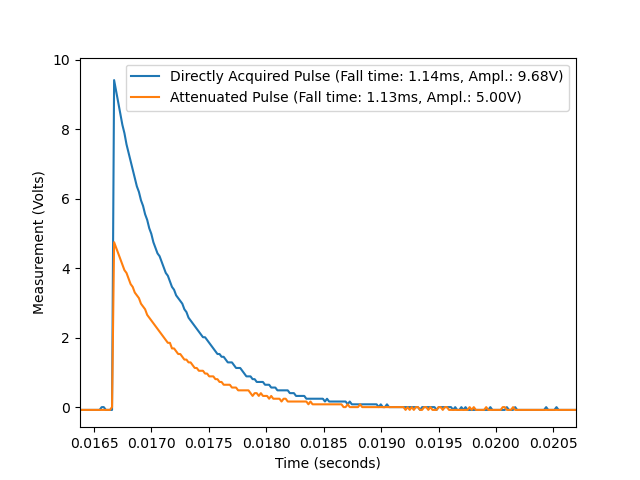
\includegraphics[width=\figwidth]{figs/Exp2_dir-v-att_zoom.png}
    \caption{A sample waveform of two different outputs recorded from the Pulser, one directly acquired and one with minimal (x2) attenuation. Note how the magnitude of the 2x attenuated waveform is also approximately half that of the direct.}
    \label{fig:exp2-atten-zoom}
\end{figure}

% Experiment 3
% Plots of sample pulses for different gain and shaping settings
\subsection{Experiment 3: Preamplifier and Shaping Amplifier}
The results of adjusting gain and shaping of the Amplifier may be observed in Figures~\ref{fig:exp3-uni-low} through \ref{fig:exp3-uni-high}.
Figure~\ref{fig:exp3-uni-low} showcases the adjustment made by the amplifier when set to low gain (0.5, fine, 10 coarse) and shaping set to UNIPOLAR.
Setting the Amplifier's shaping to BIPOLAR with the same gain settings yielded a signal observed in Figure~\ref{fig:exp3-bip-low}.
Finally, returning the Amplifier shaping to UNIPOLAR, and using the coarse gain setting to observe a higher gain (0.5 fine, 200 coarse) yielded the much more intense signal in Figure~\ref{fig:exp3-uni-high}.
\\

The effects of adjusting Pulser gain, using the pulse height setting can be viewed in Figure~\ref{fig:exp3-ph-vs-amp}. 
Setting the pulse height setting higher resulted in higher observations both from direct Preamplifier and Amplifier outputs, but only up until a certain point. This prevented the characterization of a clear relationship $\mathrm{Amplitude = slope\times Pulser Gain + intercept}$, as noted with the certainty $R^2 = 0.574$. This relationship was quantified using the \texttt{Python} module \texttt{scipy.stats}.\\
Adjusting the Pulser pulse height setting beyond approximately 2.5 did not raise the amplitude of the Preamplifier output further, rather resulting in a distorted shape as observed in Figure~\ref{fig:exp3-broken-wave}.
Instead, increasing the pulse height setting only further distorted the waveform.
As a result, we were unable to achieve Preamplifier output greater than 25mV.
An output amplitude of less than 10mV was more typical, and increasing to 25mV required holding the Preamplifier cable taut, which will be discussed further.
\\

In Figure~\ref{fig:exp3-cg-vs-amp}, the effect of changing Amplifier gain settings on the amplitude of waves output from the Amplifier may be observed.
The lowest pulse height value on the Preamplifier (1.74) was selected and maintained while the coarse gain knob on the Amplifier was adjusted to observe the effect of amplifier gain on Amplifier output.
A clear ($R^2=0.999$) relationship $\mathrm{Amplitude = 0.315mV\times Coarse Gain + 1.246mV}$ was visible (for the constant fine gain of 0.5x)

\begin{figure}[!htb]
    \centering
    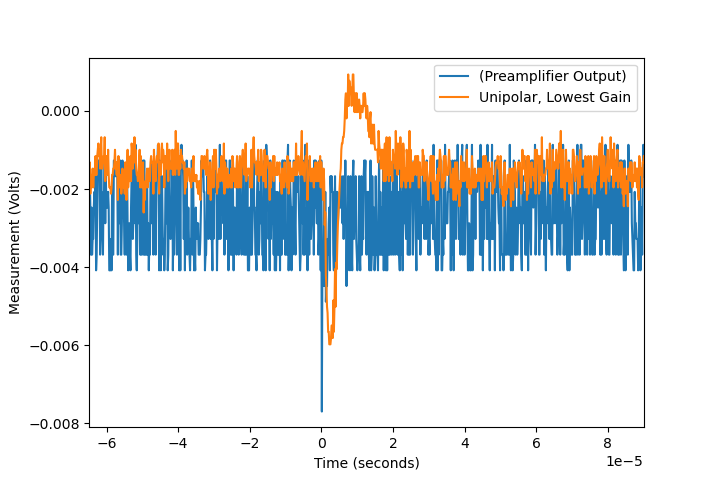
\includegraphics[width=\figwidth]{figs/Exp3_UnipolLowGain.png}
    \caption{A sample waveform recorded from the Amplifier with unipolar shaping and minimal (0.5 fine, 10 coarse) gain, compared to the direct output of the Preamplifier.}
    \label{fig:exp3-uni-low}
\end{figure}

\begin{figure}[!htb]
    \centering
    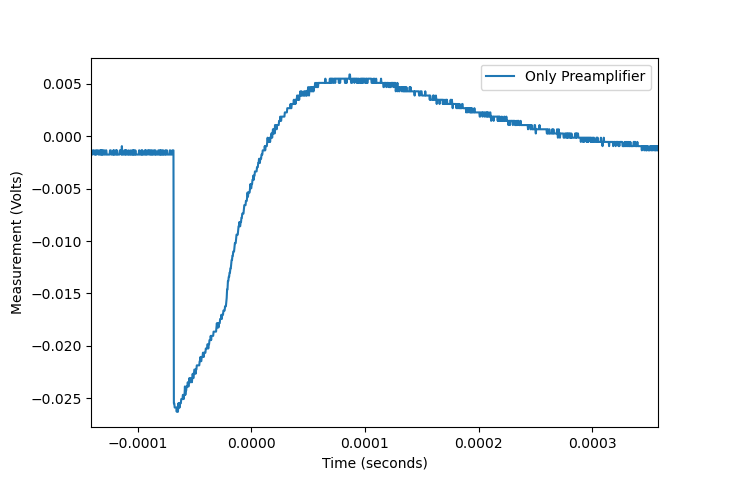
\includegraphics[width=\figwidth]{figs/Exp3_pulserPeak.png}
    \caption{The profile of a Preamplifier output wave with pulse height set beyond 2.5. Note how around -0.015V, the curve of the pulse height breaks down into a much shallower slope. Increasing the pulse height setting did not further increase this waveform's amplitude, only increasing its duration alongside the region of shallow linear slope.}
    \label{fig:exp3-broken-wave}
\end{figure}

\begin{figure}[!htb]
    \centering
    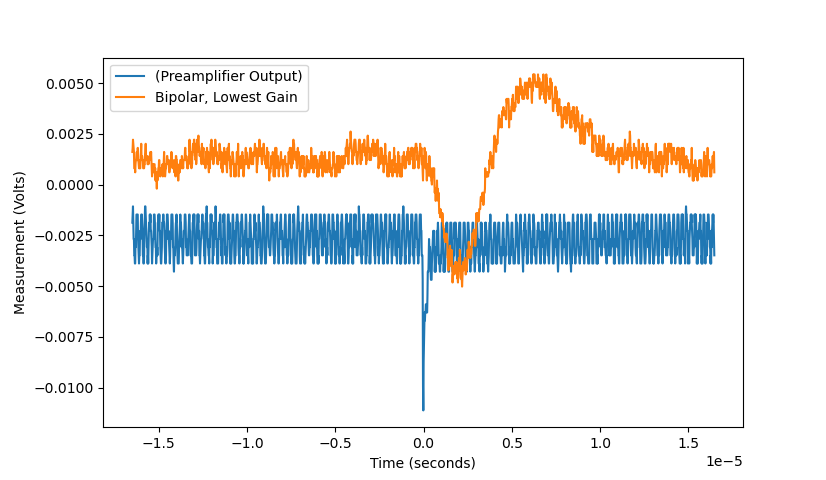
\includegraphics[width=\figwidth]{figs/Exp3_BipolLowGain.png}
    \caption{A sample waveform recorded from the Amplifier with bipolar shaping and minimal (0.5 fine, 10 coarse) gain, compared to the direct output of the Preamplifier.}
    \label{fig:exp3-bip-low}
\end{figure}

\begin{figure}[!htb]
    \centering
    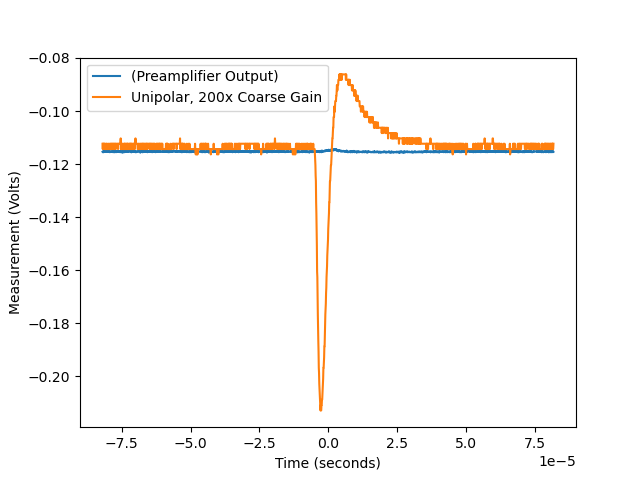
\includegraphics[width=\figwidth]{figs/Exp3_UnipolHighGain.png}
    \caption{A sample waveform recorded from the Amplifier with bipolar shaping and higher (0.5 fine, 200 coarse) gain, compared to the direct output of the Preamplifier.}
    \label{fig:exp3-uni-high}
\end{figure}

% Plots of amplitude vs gain
\begin{figure}[!htb]
    \centering
    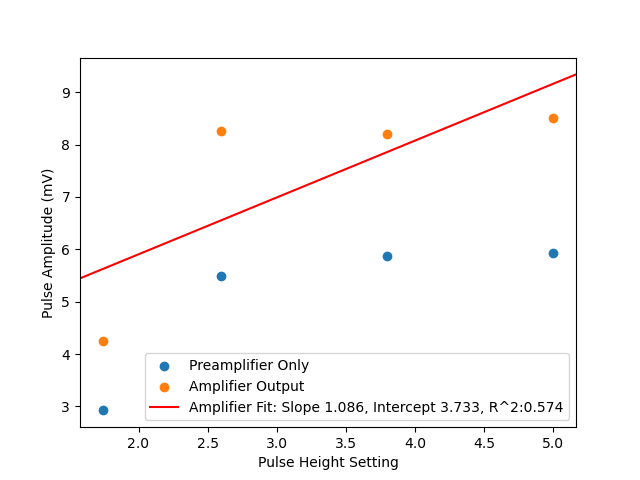
\includegraphics[width=\figwidth]{figs/Exp3_pulseHeightVsAmplitude.png}
    \caption{The recorded amplitudes (both from Amplifier output and Preamplifier directly) for various pulse height settings on the Pulser. For all signals, Amplifier fine and coarse gain were held at 0.5 and 10, respectively.}
    \label{fig:exp3-ph-vs-amp}
\end{figure}

% Plots of amplitude vs shaping parameter 
\begin{figure}[!htb]
    \centering
    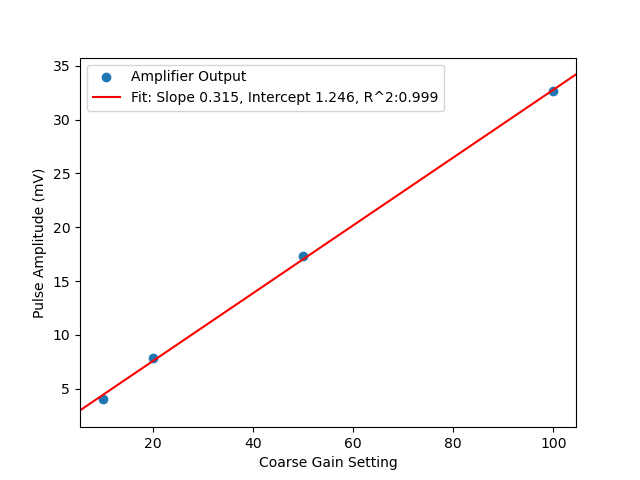
\includegraphics[width=\figwidth]{figs/Exp3_coarseGainVsAmplitude.png}
    \caption{The recorded amplitude of the Amplifier output signal for various coarse gain settings of the Amplifier. For all signals, fine gain was held at 0.5 and pulse height on the Pulser held to 1.74.}
    \label{fig:exp3-cg-vs-amp}
\end{figure}
Because of issues with the Preamplifier, we were unable to subsequently achieve a pulse of 100mV using only the Pulser gain (pulse height setting).
At the discretion of the TA, a coarse gain of 200 was used instead of 10, allowing a pulse height of 100mV to be recorded.
After changing the signal inputs of the Oscilloscope from Preamplifier output and Amplifier AMP output to Amplifier AMP and SCA outputs, the SCA signal was observed to have a pulse width of 8 microseconds (compared to AMP signal of 21 microseconds), a magnitude of 887.5mV (compared to the 100mV targeted with the AMP output), and a pulse frequency of 60.06Hz (identical to AMP output.)

% Written explanation of observed results

% Experiment 4
% Written explanation
\subsection{Experiment 4: The Timer-Counter}
Using the configuration shown in Figure~\ref{fig:mat-exp4-setup}, the AMP output of the Amplifier, with a UNIPOLAR shaping setting was fed to the Counter.
The Counter was set to record for 60 seconds, after which a count of 3598 was observed, yielding a frequency of $Nt^{-1}=3598\times(60[s])^{-1}=59.967$Hz, approximately equal to the pulse frequencies of 60.06Hz previously observed.
% Experiment 5
% Written explanation
\subsection{Experiment 5: Discriminator}
Using the configuration shown in Figure~\ref{fig:mat-exp3-setup2},
the AMP and SCA outputs of the Amplifier were connected to the oscilloscope.
Using the Pulser gain and maximizing both dials of the Amplifier gain, an output pulse with magnitude of 0.8825 was observed.
With the Lower Level Discriminator (LLD) set to a minimum value and the Upper Level Discriminator (ULD) to a maximum value while the Amplifier SCA was set to WINDOW, the logic pulse from the SCA output was clearly visible.
With ULD maximized, the LLD could be increased to a maximum of 0.26 before the wave was fully discriminated (no SCA logic pulse visible for any AMP waveform), with flickers starting as low as 0.16. 
Conversely, with LLD minimized, the ULD could be lowered to a minimum of 0.06 before the wave was fully discriminated, with flickers starting as high as 0.1.
\\

While changing the LLD and ULD of the Amplifier in WINDOW SCA mode caused the SCA's output logic pulse to either trigger or not trigger on a pulse from the AMP output (as described above), changing these window settings did not affect the AMP output signal of the Amplifier, only how the SCA output signal was generated in response.

If the SCA signal was used instead of the AMP output in experiment 4, a similar result may have been observed, but if the Discriminator settings were not properly adjusted then the Counter could have counted fewer or more pulses than were actually measured (either from over-discriminating, or by allowing measurement of noise, for example), resulting in an inaccurate frequency measurement.

\section{Discussion}\label{sec:disc}
The results of experiments 1 and 2 illustrate a comprehensive degree of control over the Oscilloscope display, how the Oscilloscope detects repeating waves, and the ability to record signal information like amplitude, duration, and frequency.\\

The results of experiment 2 also illustrate the ability to control the output signal of the Pulser to achieve pulses of certain amplitudes, as well as the ability to output before and after attenuation, allowing very direct control over this "debug" signal to ensure a sufficiently high-magnitude output with minimal noise.\\

When using the Pulser directly, there were some issues with noise, and with shape.
We had difficulty increasing the 
For example, an attenuation of "10x" was initially used, but after encountering difficulty setting an appropriate Trigger to avoid noise, this was then switched to the more moderate "2x" to center on a clear waveform and record this data, and allow the plotting as in Figure~\ref{fig:exp2-atten-zoom}.\\

The results of experiment 3 demonstrate the degree of control over the Amplifier, and how it modifies the signal of the Preamplifier.
The shape of the signal could be altered, and could be altered in different ways by changing the shaping parameter.
The magnitude of the signal could be amplified to a degree changed using the gain settings of the Amplifier, and this was found to be more reliable
than changing the Preamplifier gain.
Where changing the Preamplifier gain using the pulse height dial could only amplify the signal to a limited extent, a very clear ($R^2=0.999$) linear change was made to Amplifier output by changing the Amplifier's gain settings. \\

It is unclear how much of this is typical of normal amplifiers and pulsers, however, given the issues found (confirmed by both TAs) with the Preamplifier used.
The connection to the Preamplifier was extremely loose, and this both reduced the amplitude of the output signal and introduced a great deal of noise into the signal, especially in conjunction with a t-splitter.
This is most visible in the direct comparisons like in Figure~\ref{fig:exp3-uni-low}.\\

This effect limited the readability and control over outputs using the Preamplifier output, and in particular seemed to hinder the maximum voltage reached without amplification.
These were only partly resolved, but at least made somewhat consistent, by having a lab member hold the Preamplifier output cable taut at all times, and after these three sample wave measurements directly comparing the waveforms of Preamplifier and Amplifier output were recorded, further measurements were taken separately for Preamplifier and Amplifier output, without using the t-splitter.\\


The results of experiment 4 demonstrate the ability to fairly reliably record the number of signals within a set timeframe, as the counts measured were nearly exactly what was expected from the previously measured frequency.
This does, however, assume the input signal were calibrated appropriately: for example, in a first attempt, the SCA output signal sent from the Amplifier to the Counter was inverted, resulting in a 60-second count of $7194$, nearly twice what was expected.\\


The results of experiment 5 demonstrate control over waveform discrimination, allowing discrimination against signals either too small or too large, or just against signals too small.
The importance of selecting appropriate ranges was demonstrated through the ease of discriminating our target SCA output pulse, either entirely or even partially (the flickering), which would be even harder to address.\\

Experiment 5 also demonstrated the issues with the Preamplifier, as even when maximizing Amplifier and Pulser gains, we were unable to obtain an SCA logic pulse of 1V (At most 0.8825V).
\section{Conclusions}\label{sec:conc}
The objectives of the lab\cite{npre_lab_1_manual_2025} were mostly met.
We demonstrated ability to form and debug simple NIM systems to detect radiation.
In particular, ability to use the Pulser to produce controlled sample pulses, the Oscilloscope to view and measure repeating pulses, the Preamplifier and Amplifier to enhance, amplify, shape, and discriminate pulses, the Counter to count signals over a time period, and BNC cables to connect different components, was demonstrated.
We recorded the effects of different controls for the Oscilloscope.
This will allow signal processing to be more effectively debugged and designed in future laboratories by easily comprehending the signal output.
We recorded sample waveforms from the Pulser directly, then with the Preamplifier and Amplifier processing Pulser signal, with different configurations of gain and shaping from the Amplifier.
This will allow future systems to be more easily debugged with behavior following predictable repeated pulses, and the more reliable processing of signals using a comfortable control of a preamplifier and amplifier.
We were able to generate an SCA pulse with a measured width of 8 microseconds, magnitude 0.8875V, and frequency 60.06Hz, compared to a corresponding AMP pulse of 21 microseconds, 100mV, and identical 60.06Hz.
Using the Counter, we measured 3598 pulses in 60 seconds, an extremely similar frequency of 59.96Hz.
This demonstrates both the usability of the Counter for future experiments, but eases its validation through configuration of signals which can be tested for frequency on an oscilloscope.
We found a much more reliable control over amplification with the Amplifier ($R^2=0.999$) than using the Pulser gain and Preamplifier directly ($R^2=0.574$), though this might in part be attributable to Preamplifier difficulties.
This may suggest for future experiments to focus on configuring amplifier gain, if possible.
We found that for an SCA pulse of amplitude 0.8825V, an LLD of at most 0.26, or separately a ULD of at most 0.06 were required to guarantee false discrimination of the target signal.
This reinforces our caution with discriminating signals, as it is both necessary to discriminate against noise and easy to accidentally discriminate target signals, in part or in whole.\\

While there were equipment difficulties, the impact of these on lab completion was minimal: Output attenuation was demonstrated at 2x instead of 10x for the Pulser, a signal of 100mV was only achieved in experiment 3 using Amplifier gain and not just Pulser gain, and a maximum SCA pulse amplitude of 0.8875V was created.
Perhaps most significantly, the effect of Pulser gain on resulting pulse amplitude was hard to quantify due to the unexpected plateauing of pulse amplitude. 
Were we to repeat this laboratory, the replacement of the Pulser or Preamplifier used might improve the usability of results, though in both cases it was possible to work around issues.

% \bibliographystyle{sty/ieeetran}
\printbibliography
\end{document}
